\subsection{External interface requirements}
\subsubsection{User interfaces}
This section puts focus on the relation between the user and the mobile application. For better understanding the set of functionality of the application and the interaction with the user, beneath there are some mockups that represent a basic idea of what the mobile app will look like.

\begin{center}
\begin{minipage}[c]{.40\textwidth}
\centering
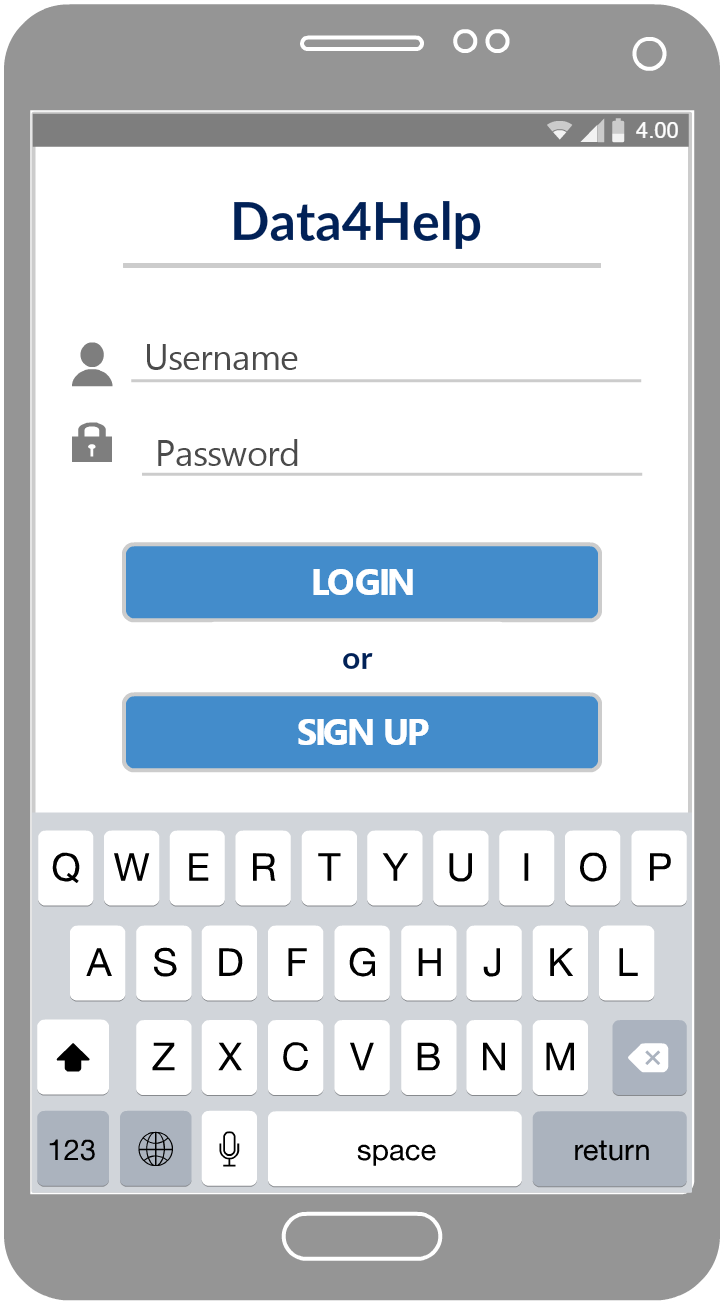
\includegraphics[width=1\textwidth]{Images/userInterface/Login}
\captionof{figure}{Mock up: Login.}
\end{minipage}%
\hspace{10mm}%
\begin{minipage}[c]{.40\textwidth}
\centering
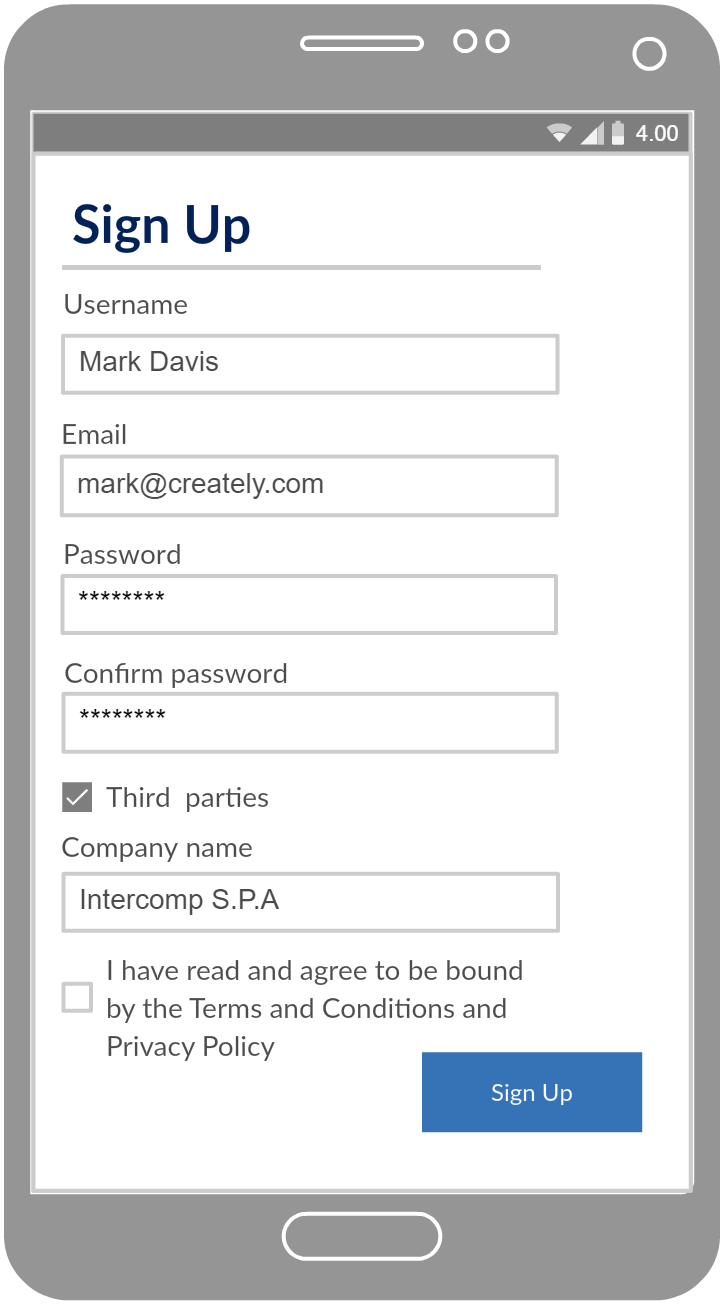
\includegraphics[width=1\textwidth]{Images/userInterface/SignUp}
\captionof{figure}{Mock up: Sign up.}
\end{minipage}
\end{center}
  
\begin{center}
\begin{minipage}[c]{.40\textwidth}
\centering
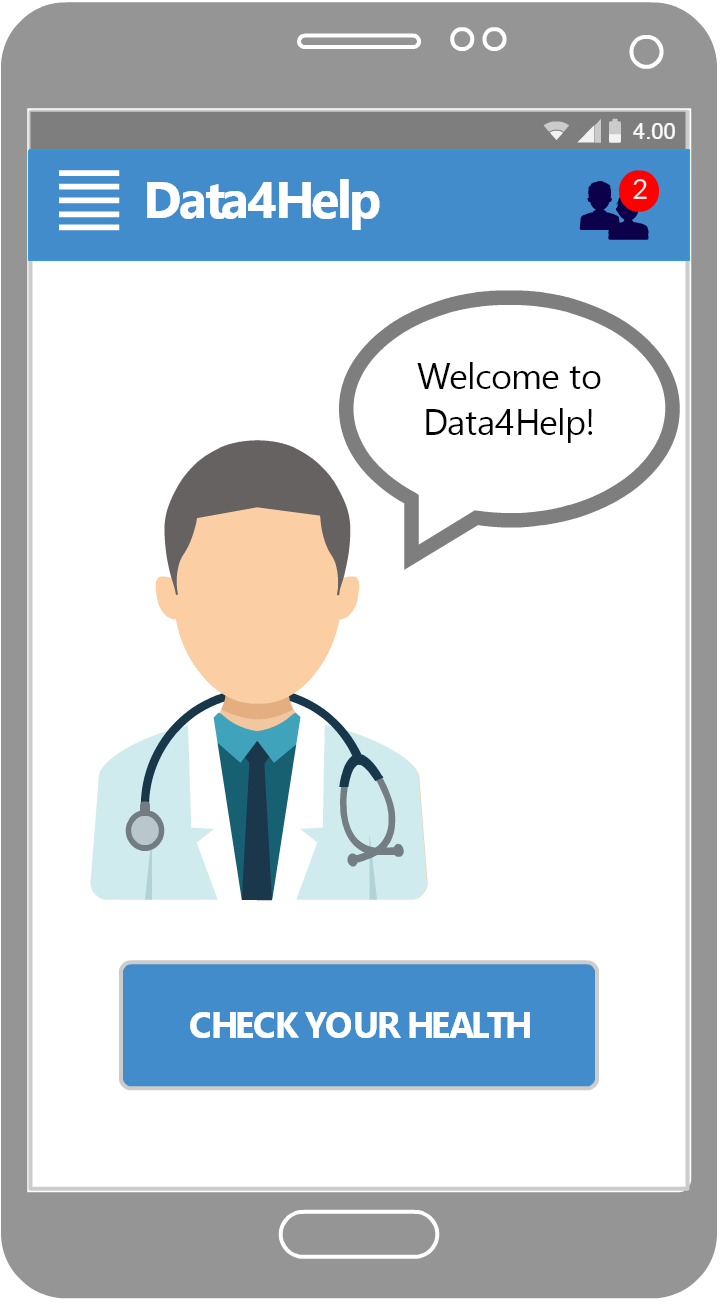
\includegraphics[width=1\textwidth]{Images/userInterface/Home}
\captionof{figure}{Mock up: Home.}
\end{minipage}%
\hspace{10mm}%
\begin{minipage}[c]{.40\textwidth}
\centering
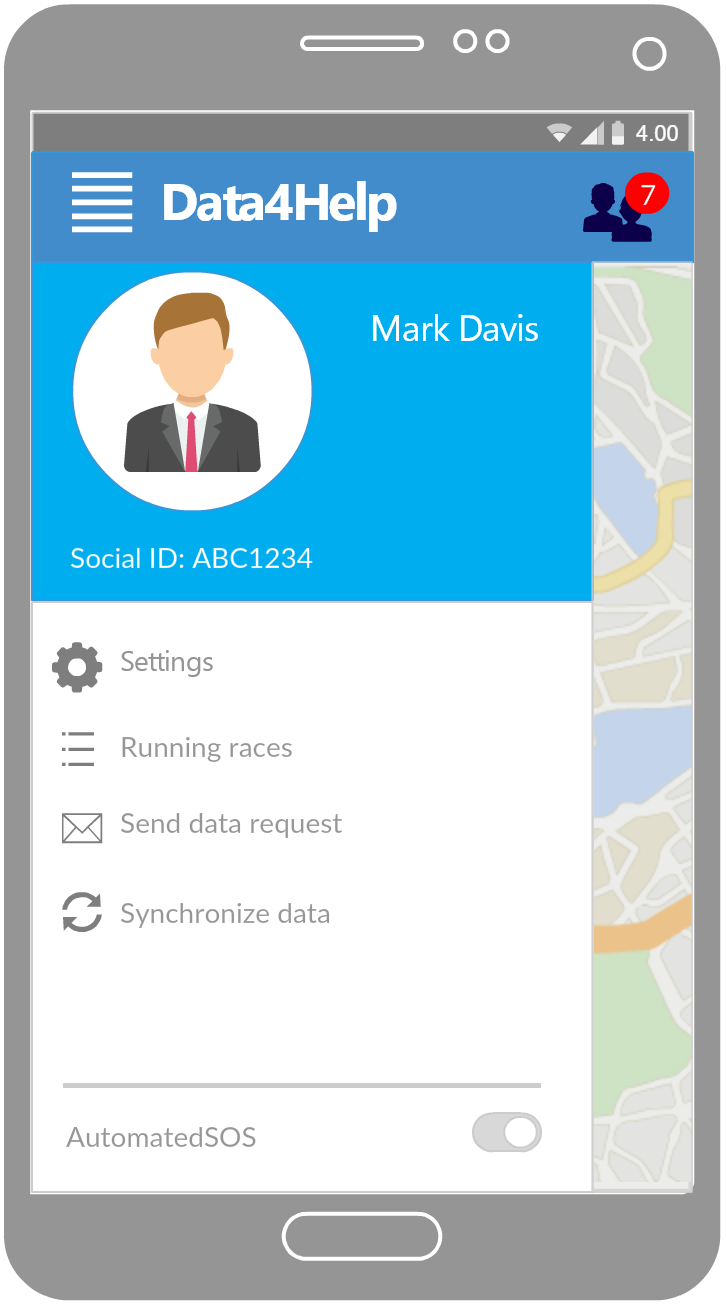
\includegraphics[width=1\textwidth]{Images/userInterface/MainMenu}
\captionof{figure}{Mock up: Main menu.}
\end{minipage}
\end{center}

\begin{center}
\begin{minipage}[c]{.40\textwidth}
\centering
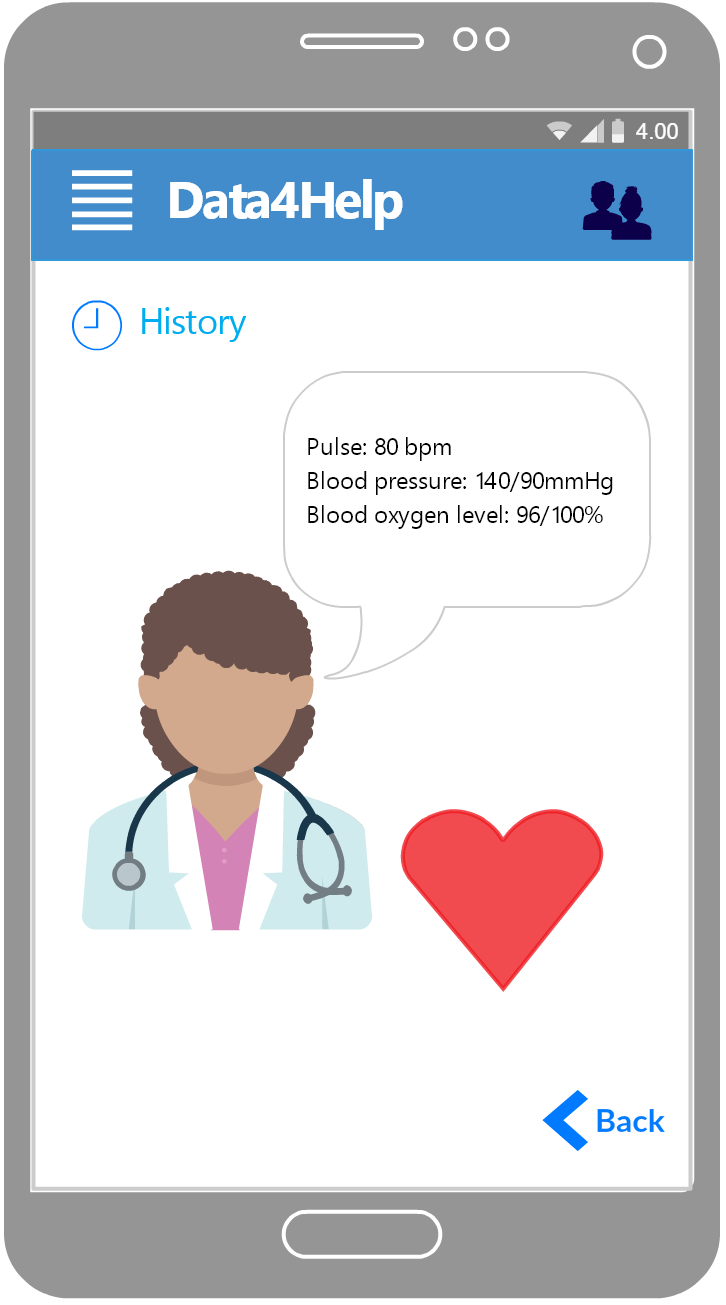
\includegraphics[width=1\textwidth]{Images/userInterface/HealthStatus}
\captionof{figure}{Mock up: Health status.}
\end{minipage}%
\hspace{10mm}%
\begin{minipage}[c]{.40\textwidth}
\centering
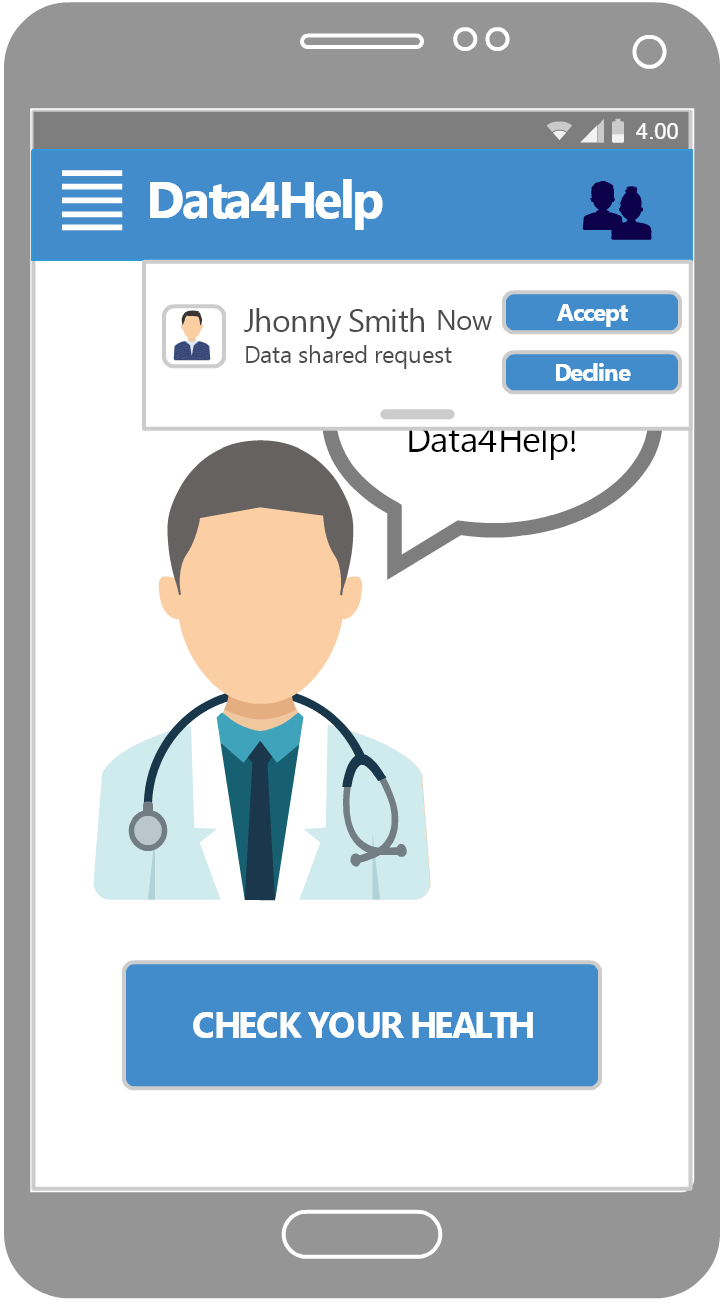
\includegraphics[width=1\textwidth]{Images/userInterface/ManageRequest}
\captionof{figure}{Mock up: Manage the request.}
\end{minipage}
\end{center}

\begin{center}
\begin{minipage}[c]{.40\textwidth}
\centering
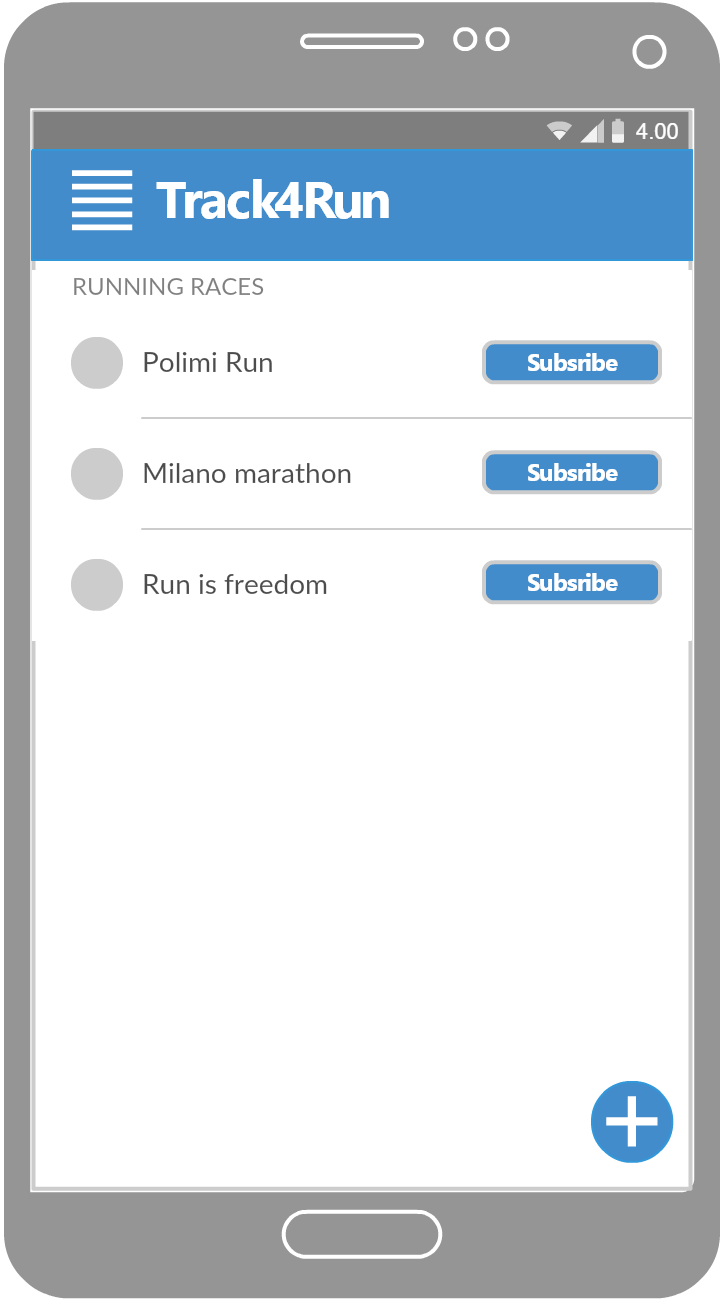
\includegraphics[width=1\textwidth]{Images/userInterface/RaceList}
\captionof{figure}{Mock up: List of available races.}
\end{minipage}%
\hspace{10mm}%
\begin{minipage}[c]{.40\textwidth}
\centering
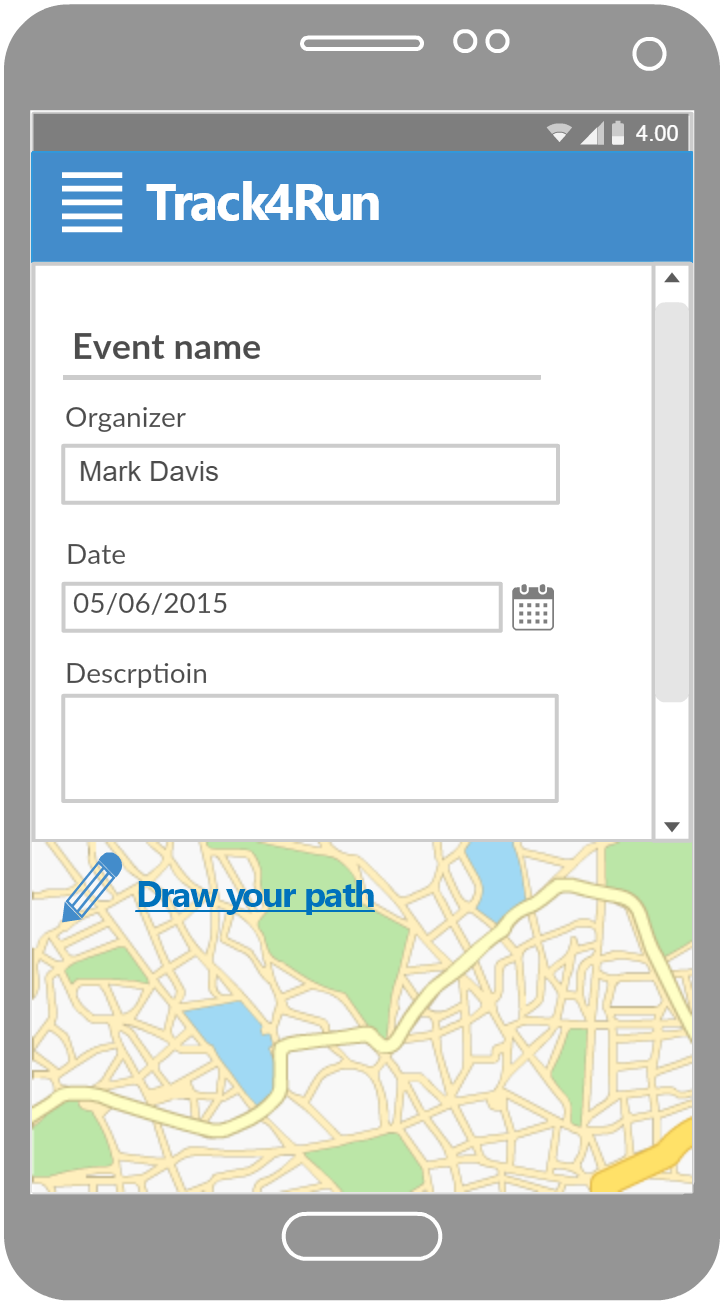
\includegraphics[width=1\textwidth]{Images/userInterface/AddEvent}
\captionof{figure}{Mock up: Add some events.}
\end{minipage}
\end{center}

\begin{center}
\begin{minipage}[c]{.40\textwidth}
\centering
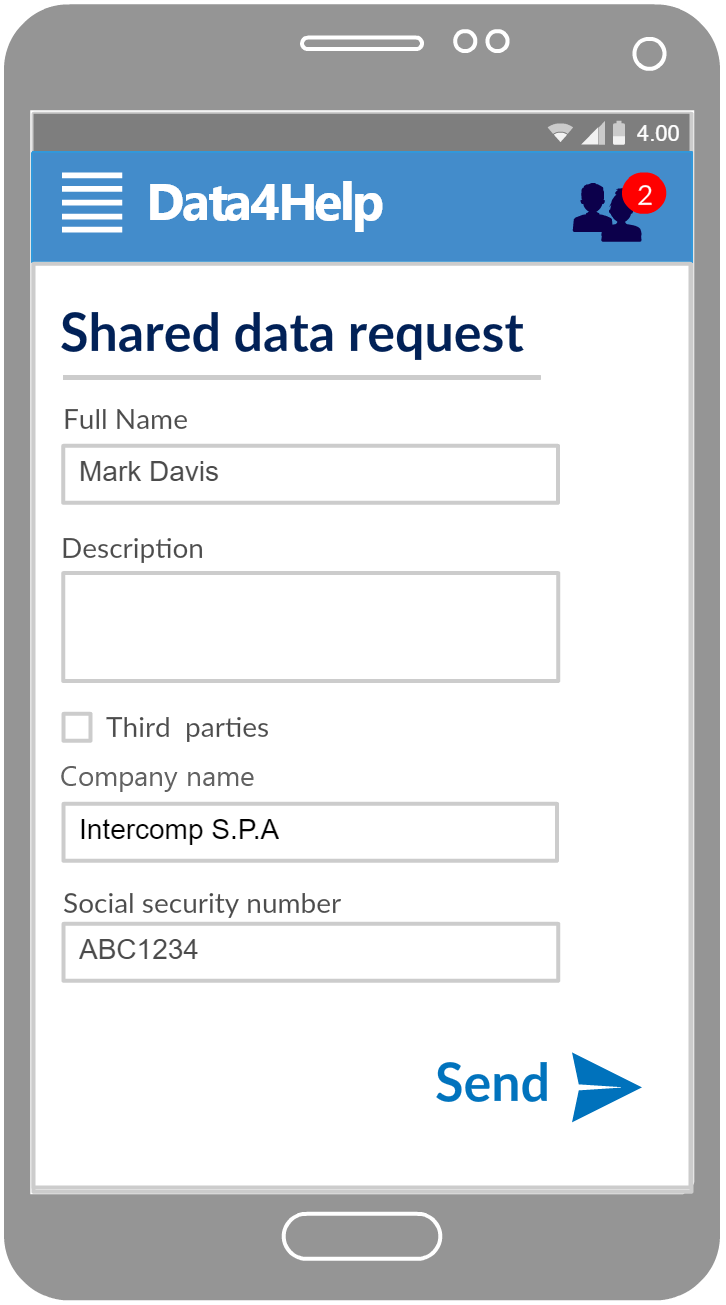
\includegraphics[width=1\textwidth]{Images/userInterface/SendRequest}
\captionof{figure}{Mock up: Shared data request form.}
\end{minipage}%
\hspace{10mm}%
\begin{minipage}[c]{.40\textwidth}
\centering
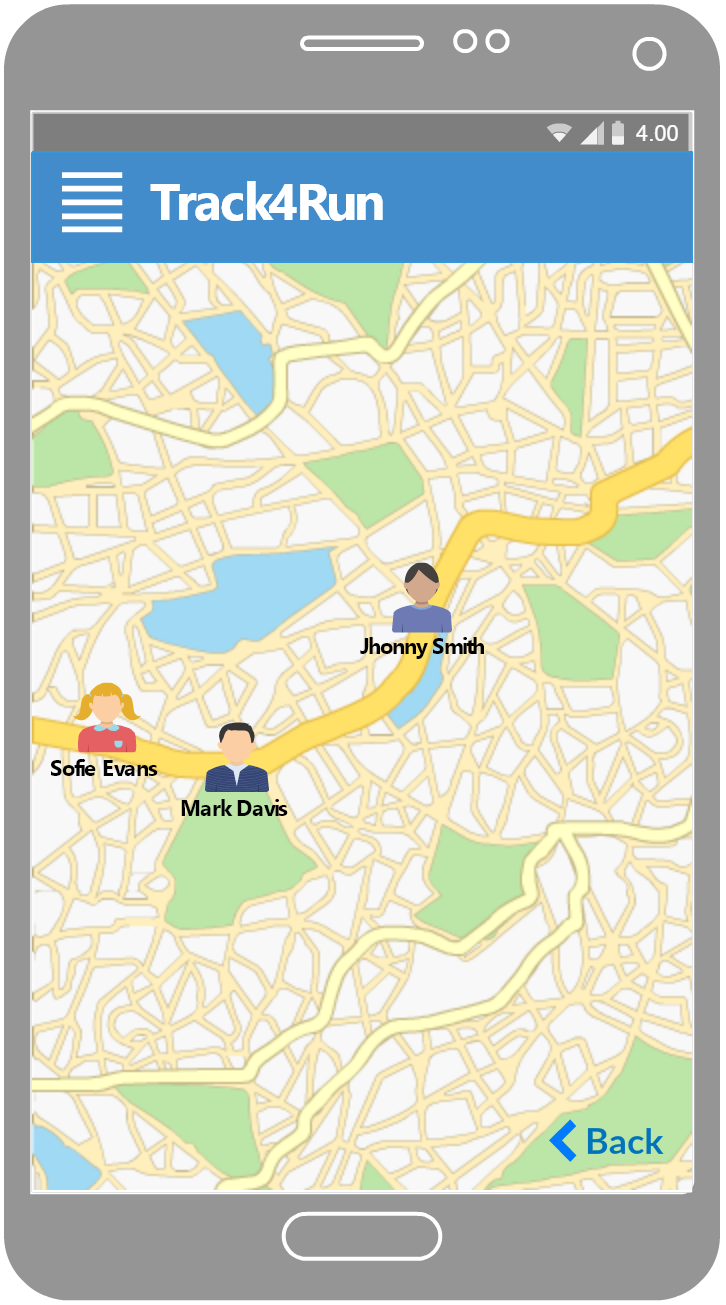
\includegraphics[width=1\textwidth]{Images/userInterface/Race}
\captionof{figure}{Mock up: Competition view.}
\end{minipage}
\end{center}


\subsubsection{Hardware interfaces}
To exploit the set of functionality of TrackMe services is mandatory to have two distinct hardware components:
\begin{enumerate}
\item First, it is necessary to own a smartphone which is used to interact with the mobile application;
\item Second, it is also essential to have a device provided with at least one NFC sensor: this has the ability to acquire heartbeat, blood pressure and blood oxygen saturation levels data.
\end{enumerate}
The latter, other than data acquisition, is also able to communicate with the smartphone in order to send the data acquired.\\
\begin{figure}[h!]
  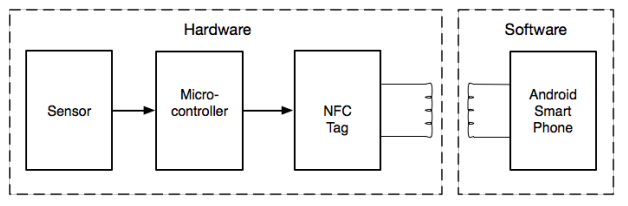
\includegraphics[width=\linewidth]{Images/hardware}
  \caption{Example of System Architecture.}
  \label{fig:The System Architecture}
\end{figure} 
The smartphone must also have a GPS system to provide the position, a monitor to allow, during the race, to see the athletes on the path, and finally the phone must be able to call the emergency room number.

\subsubsection{Software interfaces}
The application uses external services to reduce the product complexity:
\begin{enumerate}
\item Race map\\
The application requires the usage of maps to define a path for a race and to see the position of the athletes during the competition. One option here is using Google Maps API which lets customize maps with owner content and imagery.
\item Call service\\
The smartphone's call service installed on the device is used by the application due to call the emergency number.
\item GPS Data service\\
The GPS Data as a Service API allows developers to store, handle, and manage GPS data in the system. It also analyzes GPS data in real time so that application can use it to provide the position during the call to the emergency room operator and during the running race.
\item Automated call\\
Automated call service allows, to AutomatedSOS, to call the emergency number and to speak with the operator.
For instance, an option to recognize the answer provided by the emergency room operator could be the Google Cloud Speech API, that enables the AutomatedSOS feature to convert audio to text by applying neural network models in an easy to use API. 
\item Text-to-speech\\
The Text-to-Speech API is ideal for any application that plays audio of human speech to users. It allows the application to convert arbitrary strings, words, and sentences into the sound of a person speaking the same things. For example, in this case the API is used to read a formatted text message during the call to the emergency number. The message provides all the information that usually are required by the health staff. One possible API for this interface can be Google Text-to-speech.
\end{enumerate}


\subsubsection{Communication interfaces} 
The project needs several communication interfaces:
\begin{enumerate}
\item A communication interface to read/write data from the NFC tag. Fortunately, this already exists and it is called NFC protocol.
\item A communication interface to send and receive data over the network, in order to interact with the TrackMe system. One possible solution is to use the protocol HTTPS, that guarantees data security during upload and download operations. 
\item A communication interface to perform calls. 
\item A communication interface that exploits the GPS technology
\item A communication interface between mobile application and the NFC device to transfer the collected data
\end{enumerate} 
